\documentclass{article}
\usepackage{graphicx}
\usepackage{float}
\usepackage[utf8]{inputenc}
\usepackage{csquotes}
\usepackage{cleveref}
%\usepackage{biblatex}


\setlength{\parindent}{0cm} %Indenteringen för första raden på ett nytt stycke
\setlength{\parskip}{3mm} %Avståndet för en ny rad inom samma section
\setlength{\hoffset}{-40pt} % Flyttar vänstermarginalen -70
\setlength{\textwidth}{430pt}

\begin{document}
	
\pagenumbering{<command>}
\pagenumbering{Roman}
	
\title{Automatic detection and localization of relatively permanent pigmented or vascular skin marks}
\author{Armand Moulis}
\date{\today}
\maketitle

\newpage

\listoffigures

\listoftables

\newpage

\setcounter{tocdepth}{3}
\tableofcontents

\newpage

DETTA KOMMER ATT TAS BORT NÄR VÄL RAPPORTEN ÄR KLAR. KAN DOCK VARA AV INTRESSE UNDER TIDENS GÅNG 
\section*{Document history}
\begin{center}
	\begin{tabular}{|l|l| p{5cm} |l|l| }
		\hline
		Version & Date   & Changes & Sign & Reviewed \\ \hline
		0.1     & \today &         &      &  \\ \hline
	\end{tabular}
\end{center}


%% Start of the document

\section*{Abstract}

\textit{Keywords:} facial marks, 

\setcounter{page}{1}
\pagenumbering{arabic}
\newpage


\chapter{Introduction}\label{cha:intro}
\section{Motivation}

The amount of video surveillance cameras, security cameras and cellphone cameras increases rapidly and today there exist millions of devises capable of catching perpetrators in the act. The videos and still images can be
used as evidence for identification during trials where forensic experts evaluate the strength of evidence whether if the suspect is the same person as the one caught
on camera.

%The amount of technical tools available for forensic analysis in law enforcement increases rapidly and today there exist millions of devises capable of taking colour images. Video surveillance cameras, security cameras and cellphone cameras can all be used to catch perpetrators in the act. The videos and still images can be used as evidence for identification during trails which means that forensic technicians need tools to evaluate if the suspect is the same person as the one caught on camera.

One common method of evaluating whether the perpetrator and the suspect are the same person is to compare facial features such as eyes, nose, mouth, scars, and other facial marks. This is nowadays done manually \cite{face_soft} by the forensic examiners, and in order to evaluate the strength of the results, a likelihood ratio \cite{NFC_stat} from Bayes rule is calculated. The likelihood ratio is estimated from two hypotheses, where the numerator gives the probability to achieve the results 
if the perpetrator and the suspect are the same person and the denominator the probability to achieve the results if the perpetrator is another man. 

National Forensic Centre (NFC) is currently running a project where an automatic facial recognition system can be used to extract statistics from a database of facial images. The main advantages of using such a method are that the likelihood ratio can be calculated based on statistics, and that the risk for human bias in the decision process is diminished.

%To calculate the likelihood ratio it is required to have enough observations of facial features and these are acquired manually by experts since facial recognition processes have not been found to be reliable enough \cite{automatic_detector_2015}. To record all these observations manually is time consuming and there exist a interest in doing this automatically \cite{forensic_identification}. 
This master thesis was motivated by the need of combining the automatically calculated likelihood ratio value with the evidential value derived from the frequency of facial marks in certain regions of the face. The NFC in Sweden is supporting this work by providing guidance and practical help.

%This master thesis was motivated by the need of large amount of data from facial marks. The National Forensic Centre (NFC) in Sweden is supporting this work by providing guidance and practical help.  
\section{Aim}

The aim of thie master thesis is to create a algorithm to automatically create a large data base with facial images and their features. By using this algorithm, the evidential value in forensic facial image comparison examinations can be better grounded.

\section{Problem specification}

The problem of this master thesis is to find a method for automatically detect and locate facial marks and classify them as permanent or non-permanent marks. The frequency, location and size of the permanent marks are stored such that they can be used together with the previously calculated likelihood ratio

%This master thesis is going to answers the following questions: 
%\begin{displayquote}
%	Is it possible to implement a algorithm which can automatically detect RPPVSM?
%
%	How can the RPPVSM be given a location and size within a face?
%
%	With which accuracy can the algorithm detect and localize RPPVSM?
%\end{displayquote}



\section{Scope}

In general, when working with image, the quality of the images are crucial for the results. Low resolution and badly illuminated images taken from different angles can cause analytical difficulties. Therefore, this thesis assumes images which are high resolute, well illuminated, taken en face and in RGB-colours. 

\section{Thesis outline}

This chapter describes the aim and problem specification of this master thesis. In Chapter \ref{cha:related_work}, gives an insight in related work the methods used by other researchers. Chapter \ref{cha:method} describes the methods used in the algorithm developed during this master thesis. The results from the algorithm can be studied in Chapter \ref{cha:result} and an discussion about the result and methods used is found in Chapter \ref{cha:Discussion}. Finally, Chapter \ref{cha:conclusion} consist of a conclusion of the master thesis and ideas for future work within the same scope. 

\chapter{Theory}\label{cha:theory}

This chapter will describe the underlying theory about the methods and algorithms used during in the automatic facial mark algorithm. 

\section{Facial landmarks} \label{sec:landmarks} 

To process a facial image, it is useful to know where different parts of the face are located, e.g. mouth and eyes. These parts can be pinpointed with points called landmarks. With these landmarks, it is possible to create a unique mask for each face and produce a grid with different regions in the face. The landmarks are extracted by using an implementation based on Vahid Kazemi et al. \cite{dlib_landmark}. It uses sate of the art algorithms for face alignment where cascade of regression functions is crucial for its success. The estimated shape of the face is updated by regressing the shape parameters based on normalized features from the image. The parameters are updated until they converge.

From this algorithm, 68 landmarks are extracted where the eyes, mouth, nose and chin are marked. From these, a mask generated where the nostrils, eyes, throat and background are cut out. 

\section{Image normalization} \label{sec:normalization} 

In order to get a reliable and uniform result in the algorithm, the facial images have to be normalized. There are two kinds of normalization applied on the image, geometric normalization and photometric normalization.  

\subsection{Geometric normalization} \label{subsec:geo_norm} 
The geometric normalization consists of a rotation of the image such that the line between the pupils is aligned with the bottom of the image. The rotation angle is calculated with the help of the landmarks at the corners of the eyes. Each eye contributes with a rotation angle and the average of them is used to rotate the image.

Rotation of an image is done by using an affine transformation with homogeneous coordinates \cite{li2001generalized}. Assume that a point is described as $(x, y)$ in Cartesian coordinates. Then, the point can be transformed into homogeneous coordinates such that the point is described as $(x, y, 1)$. Thanks to this coordinate system, rotation can be expressed as a simple matrix multiplication as in \cref{eq:rotation} where $(x', y', 1)$ are the rotated coordinates for a point. Each point is rotated counter clockwise with $\phi$ degrees.

\begin{equation} \label{eq:rotation}
\begin{bmatrix}
x' \\[0.3em]
y' \\[0.3em]
1
\end{bmatrix}
=
\begin{bmatrix}
	\cos{\phi} & -\sin{\phi} & 0 \\[0.3em]
	\sin{\phi} & \cos{\phi}  & 0 \\[0.3em]
	0          & 0           & 1
\end{bmatrix}
\begin{bmatrix}
x \\[0.3em]
y \\[0.3em]
1
\end{bmatrix}
\end{equation}

The geometric normalization also includes a rescaling of the image such that the interpupillary distance is 500 pixels. A resizing factor is calculated by taking the fraction between 500 and the number of pixels between the pupils.  

\subsection{Photometric normalization} \label{subsec:photo_norm} 

The photometric normalization is performed by using a tone mapping operator based on the work of Nikola Banic et al.\cite{badger}. It uses a Light Random Sprays Retinex (LRSR) which is an improvement of the Random Sprays Retinex (RSR)\cite{RSR}. All tone mapping operators transform pixel intensities based on its surrounding. The RSR uses a random selection of pixels around the current pixel which decreases computation costs, sampling noise and dependency. The calculations are done on the intensity image of each RGB colour channels. An example of the output from the image normalization can be seen in \cref{fig:rotated_img}.

\section{Face detection}

An important component in the algorithm is the bounding box of the face in each image. It is found by using an OpenCV \cite{opencv} implementation of object detection by Paul Viola et al. \cite{face_detection}. This face detection algorithm was chosen since it shows as positive result as other methods \cite{face_detecion_comp,face_detecion_comp_2}. In addition, it is much faster the other detector. The algorithm from Paul Viola et al. take advantage of three different parts. 

The first is part is a new image representation which allows Haar features from each image to be calculated rapidly. The speed is achieved by using integral images instead of the original image. 

The second part is the extraction of the most important features through AdaBoosting. It creates a strong classifier by combining the strength of weaker classifiers. A weak classifier is the best threshold for a feature which separates faces and non-faces.

The third part is a cascade decision which reduces the computation costs by rejecting potential bounding boxes for the face. A simple classifier is used to determine if the bounding boxes are promising candidates before a more complex classifier is engaged. This is repeated until all classifiers have been passed or one of the returns a negative result. All bounding boxes which have returned a negative result is rejected immediately.  

\section{Segmentation} \label{sec:segmentation} 

When searching for facial mark, hair lines and hair can cause false detection. Therefore, the image has to be segmented so that only skin area is regarded during the search of facial marks. Since interactive segmentation methods are more and more popular \cite{graphcut}, it should be beneficial to choose an interactive segmentation method. Carsten Rother et al.\cite{grabcut} compared several popular interactive segmentation methods and also presented their own method, GrabCut. They concluded that GrabCut performs as well as GraphCut \cite{graphcut} with fewer user interactions.

Thus, the segmentation method used for the algorithm is GrabCut which uses Gaussian Mixture Model (GMM) for a color image. GrabCut needs a GMM for a known foreground and one for a known background. The known foreground used e.g. is the cheeks and forehead, is extracted with the help of the landmarks. 

After creating GMM:s, an energy function is created so that its minimum correspond to a good segmentation which depends on the given foreground and background. The function is minimized iteratively until a converged segmentation is produced.

The segmentation mask is used to improve the mask created from the landmarks. Now using the improved mask, a well segmented image can be searched for facial marks. 

\section{Fast Radial Symmetry} \label{sec:FRS} 

There are many ways to extract interesting points or marks. One way is to look at the radial symmetry in the image. This method has been used by several researcher \cite{twins,FRS,automatic_detector_2015,yeast}. It seems to be a reliable method since the point is to detect small circular shapes, which is what Jan Schier et al.\cite{yeast} did when they tried to count yeast colonies. This is why the actual mark detector uses an algorithm called Fast Radial Symmetry (FRS) and it was created by Gareth Loy et al.\cite{FRS}. 

For each point, $p$, in an image, the contribution of radial symmetry at radius $r$ is calculated by producing an orientation projection image $O_n$ and a magnitude projection image $M_n$. $n$ is a specific radius. These images needs to know the so called positively-affecting pixel, $p_{+}(p)$, and negatively-affecting pixel, $p_{-}(p)$. To find theses affecting pixels the gradient, $g$, of the image is needed and it is calculated using a 3x3-Sobel kernel. Since the gradient computations are discrete, it is necessary to average the image with a 3x3 Gaussian kernel to remove sharp edges. 

\begin{equation} \label{eq:p+}
p_{+}(p) = g(p) + \text{round}\frac{g(p)}{\norm{g(p)}}n
\end{equation}

\begin{equation} \label{eq:p-}
p_{-}(p) = g(p) - \text{round}\frac{g(p)}{\norm{g(p)}}n
\end{equation}

To retrieve the nearest integer the operation $round$ is used. The $O_n$ and $M_n$ are then updated according to \cref{eq:O+,eq:O-,eq:M+,eq:M-}

\begin{equation} \label{eq:O+}
O_{n}(p_{+}) = O_{n}(p_{+}) + 1
\end{equation}
\begin{equation} \label{eq:O-}
O_{n}(p_{-}) = O_{n}(p_{-}) - 1
\end{equation}
\begin{equation} \label{eq:M+}
M_{n}(p_{+}) = M_{n}(p_{+}) + \norm{g(p)}
\end{equation}
\begin{equation} \label{eq:M-}
M_{n}(p_{-}) = M_{n}(p_{-}) - \norm{g(p)}
\end{equation}

The radial symmetry contribution at radius n depends on $F_n$ and $A_n$ which is defined as 

\begin{equation} \label{eq:F}
F_n = \frac{M_{n}(p)}{k_n} \left(\frac{\abs{\tilde{O}_n(p)}}{k_n}\right)^{\alpha}
\end{equation}
\begin{equation} \label{eq:A}
\tilde{O}_n(p) =   
\begin{cases}
O_n(p)    & \quad \text{if } O_n(p) < k_n\\
0		& \quad  \text{ else}\\
\end{cases}
\end{equation}

$A_n$ is a Gaussian kernel with different size depending on $n$, $\alpha$ is radial strictness parameter and $k_n$ is a scaling factor. $\alpha$ is set to $2$ and $k_n$ to $9.9$ since Gareth Loy et al. deemed suitable for most applications.

The final radial symmetry image $S_n$ is given by 

\begin{equation} \label{eq:S_for_n}
S_{n} = F_n * A_n
\end{equation}

This was a calculation for radius $n$ and it desirables to use multiple radii to detect point larger than $n$. It is not necessary to use a continuous spectrum of radii according to Gareth Loy et al. The average of radial symmetry images, $S$, are then calculated as in \cref{eq:S_total}. The image S is highlighting radial symmetrical regions and suppressing regions that are asymmetrical.  

\begin{equation} \label{eq:S_total}
S =\frac{1}{N} \sum_{n=1}^{N} S_n
\end{equation}



\section{Candidate elimination} \label{sec:elimination} 

Since many facial mark candidates may be false positives, they have to be discovered and excluded. Vorder Bruegge et al. \cite{automatic_detector_2015} used three elimination methods which seemed intuitive. Size, shape and presence of hair should be good indicators if the candidate is a false detection or not. Each detected candidate is given a 30x30 area which is processed through three eliminators. 

\subsection{Blob selection} \label{subsec:blob_eli} 

Facial marks are often blob-shaped which is why the first eliminator uses a simple blob detector from OpenCV. It creates a thresholded images with connective pixels and does this with different threshold values. Each image created with a fixed threshold is put together into image which is the union of all the thresholded images. If the union does not contain a blob-shaped object, the candidate is eliminated. A blob-shaped object is defined by its circularity, inertia and convexity.  

\subsection{Hair elimination} \label{subsec:hair_eli} 

The second eliminator uses a hair removal algorithm by Tim Lee et al. \cite{dullrazor}. The algorithm smooth out hair pixels with closing operations using the three different structuring elements. The suggested structuring elements by Tim Lee et al. is larger than the one used in this implementation since their hair-structures where wider. Thus, the smaller structuring elements $T_{0}$, $T_{45}$ and $T_{90}$ were used. \\

\begin{center}
	$T_{0} =
	\left[ \begin{array}{@{}*{5}{c}@{}}
	0 & 1 & 1 & 1 & 0  \\
	\end{array} \right]  $ \quad $T_{45} =
	\left[ \begin{array}{@{}*{4}{c}@{}}
	0 & 0 & 0 & 0 \\
	0 & 1 & 0 & 0 \\
	0 & 0 & 1 & 0 \\
	0 & 0 & 0 & 0  \\
	\end{array} \right]$ \quad $T_{90} = (T_{0})^{T} $ \\
\end{center}

The closed image is generated by applying each structure element on each color channel as \eqref{eq:hair}, where $G$ is the closed image, $M$ is the image of a mark, $T_x = [T_{0}, T_{45}, T_{90} ]$ and $C$ the RGB-channels. This means that $M_c$ is a gray image of a mark where the structuring elements detect thin and small edges.    

\begin{equation} \label{eq:hair}
G_c = \abs{M_c - \max_{x}(M_c * T_x)} 
\end{equation}

$\max\limits_x(M_c * T_x)$ means that the largest pixel value from the structuring elements are pick for that color channel. In the end, the union of $G_c$ is calculated and to get a hair mask, the union is binary thresholded with $h_{hair}$. If a region contains more than a certain amount of hair pixels, it will be excluded.

\subsection{Size elimination} \label{subsec:size_eli} 

The third eliminator removes candidates depending on their size. If the candidate has an area smaller than 20 pixels or an area larger than 1000 pixels, it is eliminated. The thresholds were chosen because all annotated marks is within this interval, see \cref{fig:result_box_size}.

\FloatBarrier
\begin{figure}[!h]
	\centering
	\includegraphics[width=\textwidth/2,height=\textheight/2,keepaspectratio]{result_box_size}
	\caption{The distribution of areas from the annotated facial marks.  \label{fig:result_box_size}}
\end{figure}
\FloatBarrier

\section{Machine learning} \label{sec:machine_learning} 

Machine learning is a very popular way of determining the future or sorting object into groups, e.g. whether forecast and spam filtering. The field of machine learning is growing quickly and new and more accurate methods are developed constantly. The principle is to use data to predict the outcome. The data can be somewhat incomprehensible when the dimension is getting large and abstract. This is when computers can ease the prediction by analyzing and finding patterns in the data. 

Machine learning is divided into three groups \cite{bishop2006pattern}. 

\begin{itemize}
	\item Supervised learning \\
	The system has access to labeled data from which it can find patterns and structures
	  
	\item Unsupervised learning \\
	The system does not have access to labeled data.
	
	\item Reinforcement learning \\
	The system learns from feedback given to it in form of rewards and punishments. 
\end{itemize}

A learned system can in turn be divided into two groups. 

\begin{itemize}
		\item Classification \\
		The system tries to determine the class which an object belong to, e.g. spam filtering
		
		\item Regression \\
		The system tries to predict value from an input, e.g. predicting the temperature 
\end{itemize}

This master thesis will only focus on supervised learning and classification since the desired output is permanent or non-permanent mark and there are labeled facial mark are available.  

\subsection{Supervised learning}

Supervised learning is when one try to find a function $g$ that maps $X \to \Omega$. $X$ is a vector with $N$ samples with $M$ descriptive features \cref{eq:supervised}, see \cref{sec:features}. A binary classifier usually has $\Omega = \{-1,1\}$ which it is in this case. The function $g$ takes a set of parameters $\omega = \{\omega_1 \dots \omega_K\} $ to speed up the classification of a new sample. To train the classifier, it needs training data which is a set of samples, $X$, paired with a label, $Y$. The labels has the same values as $\Omega$. 

\begin{equation} \label{eq:supervised}
X = \{x_1 \dots x_N \} \quad \text{where} \quad x_i = \{f_{i1} \dots f_{iM} \}
\end{equation}

The choice of descriptive feature a crucial for the performance of the classifier. Avrim L. Bluma et al. \cite{blum1997selection} point out importance of finding relevant and strong features. It is very easy to access to huge amount of low-quality data on the Internet. It is not the number of features that decide the performance of a classifier but rather the relevance of feature and samples. 

To illustrate how a learning method works, we jump right to a specific learning method called Support vector machine (SVM) \cite{cortes1995support}, see \cref{section:SVM} . There exist several other learning methods such as decision tree \cite{loh2011classification}, nearest neighbor \cite{keller1985fuzzy}, neural network \cite{kohonen1988introduction} and many more. This master thesis will use SVM since it is simple to use and it performed best \cite{torso_RPPVSM} compared to decision tree and nearest neighbor when classifying RPPVSM and non-RPPVSM.  


\subsection{Support vector machine} \label{section:SVM}

The principle behind SVM is to separate classes with a simple line (2D) or hyper plane (higher dimension). The line and plane can be described by its normal which has the parameters $\omega = \{\omega_1 \dots \omega_K\}$ and fulfill the equation of the plane \cref{eq:plane} where $x$ is a point on the plane and $b$ describes the distance from origin. 

\begin{equation} \label{eq:plane}
\omega^T \bullet x + b = 0 
\end{equation}

The challenge now is to find the best $\omega$ which separate the classes with the largest margin. The first attempt is a linear SVM.

\subsubsection{Linear SVM}

Vapnik et al.\cite{vapnik1963pattern} developed the linear SVM and it works like follows. Given a set of $N$ samples, $X = \{x_1 \dots x_N\}$, one want to find the normal vector $\omega = \{\omega_1 \dots \omega_K\}$ of the hyperplane which separates the two classes with the largest margin. By setting up a set of equations \cref{eq:linear_SVM} where $x_s$ is one of the samples closes to the hyperplane, so called support vector. $z_p$ is a point on the hyperplane (not a sample), $\epsilon$ is the perpendicular distance between the hyperplane and $x_s$ and $b$ determines the offset of the hyperplane from the origin along $w$. 

\begin{equation} \label{eq:linear_SVM}
\begin{cases}
\omega^T \bullet x_s + b =1\\
x_s = z_p + \epsilon \hat{\omega} \\
\end{cases}
\end{equation}

\begin{equation} \label{eq:linear_SVM_simple}
\begin{split}
& \omega^T \bullet (z_p + \epsilon \hat{\omega}) + b = 1  \iff 
 \epsilon \omega^T \bullet \hat{\omega} + \omega^T \bullet z_p + b = 1 \iff 
%& \backslash \omega^T \bullet \hat{\omega} = \norm{\omega} \:\:  \text{and} \:\: \omega^T \bullet z_p + b = 0  \backslash \\
\epsilon \norm{\omega} = 1
\end{split}
\end{equation} 

After some manipulation, see \cref{eq:linear_SVM_simple}, one notice that the best margin $\epsilon$ is achieved by minimizing $\norm{\omega}$ which is the same as minimizing $\norm{\omega}^2$ . When finding the maximal $\epsilon$, no samples may reside within the margin which can be expressed as \cref{eq:linear_SVM_in_margin} where $y_i$ is the class for each sample. This give the best hyperplane for the classifier where the classes are linearly separable \cref{fig:easy_class}.

\begin{equation} \label{eq:linear_SVM_in_margin}
y_i(\omega^T \bullet x_i + b) \geq 1
\end{equation} 

\FloatBarrier
\begin{figure}[!h]
	\centering
	\includegraphics[width=\textwidth*3/4,height=\textheight*3/4,keepaspectratio]{easy_svm.PNG}
	\caption{Linearly separable classes.
		\label{fig:easy_class}}
\end{figure} 
\FloatBarrier


\subsubsection{Soft margin SVM}

All classification problems are not always linearly separable. In this case, \cref{eq:linear_SVM_in_margin} does not hold true for all samples. This is solved by introducing a penalty $\zeta$ \cite{cortes1995support} for each sample on the wrong side of the hyperplane. This type of SVM is called a soft margin SVM. In this type, one try to solve \cref{eq:soft_SVM} where $C$ is a parameters set before optimization. 

\begin{equation} \label{eq:soft_SVM}
\underset{\omega,b,\zeta}{\mathrm{\argmin}} 
\begin{pmatrix}
\norm{\omega}^2 + C\sum_{i}\zeta_i
\end{pmatrix}
\end{equation} 

under the condition \cref{eq:soft_SVM_2}

\begin{equation} \label{eq:soft_SVM_2}
y_i(\omega^T \bullet x_i + b) \geq 1 - \zeta \quad \zeta \geq 0
\end{equation} 

Large values on $C$ results in a greater penalization for wrongly classified samples. This parameter makes a tradeoff between having a large margin and allowing samples to be on the wrong side of the hyperplane.    

\FloatBarrier
\begin{figure}[!h]
	\centering
	\includegraphics[width=\textwidth*3/4,height=\textheight*3/4,keepaspectratio]{soft_svm.PNG}
	\caption{Classes separated by a soft margin SVM.
		\label{fig:soft_class}}
\end{figure} 
\FloatBarrier

\subsubsection{Non-linear SVM}

Things are not always as simple as the case in \cref{fig:easy_class,fig:soft_class}. The classes are often not linearly separable at all. Fig. \ref{fig:hard_class} illustrate the so called XOR problem \cite{yu2012svm}. This classification problem requires a non-linear SVM. Boster et al. \cite{boser1992training} presented a way to solve the XOR problem by mapping the samples onto a higher dimension. This is done by using kernels, $k(x_i,x_j)$, of different types \cite{yu2012svm}. The following are popularly used kernels: 

\begin{itemize}
	\item Polynomial: $k(x_i,x_j) =(x_i \bullet  x_j + 1)^d $
	\item Radial Basis Function (RBF): $k(x_i,x_j) = exp(-\gamma \norm{x_i - x_j}^2 $
	\item Sigmoid: $k(x_i,x_j) =\kappa x_i \bullet  x_j + c$
\end{itemize}

where $\gamma$, $d$, $\kappa$ and $c$ are parameters set by the user. This master thesis will only use the RBF kernel since it is easy to tune and the polynomial kernel has more hyperparameters which influence the complexity of the model \cite{svm_guide}. The $\gamma$ parameter defines how far the influence of a sample reaches, a small value meaning 'far' and vice versa. Read more about kernels in \cite{vert2004primer} 

\FloatBarrier
\begin{figure}[!h]
	\centering
	\includegraphics[width=\textwidth*2/4,height=\textheight*2/4,keepaspectratio]{hard_svm.PNG}
	\caption{XOR problem with two classes. 
		\label{fig:hard_class}}
\end{figure} 
\FloatBarrier

\subsection{Overfitting}

A large number of parameters makes it possible to produce overly complicated boundaries if the training data is used for validation. This together with usage of training data as validation data can produce a problem in machine learning known as overfitting. In \cref{fig:overfitting} one can see that the red curve is a overfitted boundary while the green curve separates the two classes more generally. Overfitting occurs when the classifier tries to include outliers or wrongly labeled samples within the classifier boundary. To avoid this, one should use a subset of all the samples as testing data which will indicate if the classifier is overtrained. 

\FloatBarrier
\begin{figure}[!h]
	\centering
	\includegraphics[width=\textwidth*2/4,height=\textheight*2/4,keepaspectratio]{Overfitting.PNG}
	\caption{Example of a overfitted boundary (yellow) and a more general boundary (green). 
		\label{fig:overfitting}}
\end{figure} 
\FloatBarrier

\section{Features descriptors} \label{sec:features}

A feature descriptor extract information about patterns in an image, in this case a facial mark. This information can consist of colors in the image, edges for distinguishing light and dark areas, the texture of a surface and the direction of movement. The feature descriptors HOG, \cref{subsection:HOG}, and LBP, \cref{subsection:LBP} are common descriptors when working with detection of objects \cite{pedestrian_detection,vehicle_hog,facedetection_LBP} which is why these feature are used. Since facial marks mostly differ in color rather than shape \cite{torso_RPPVSM}, it would be wise to use features which are based on the color of the skin marks. RGB and HSV, \cref{subsection:RGB_HSV}, are primitive color-mapping but has been used a feature descriptors before \cite{torso_RPPVSM}. It would be even better to use more colors than just RGB and HSV color space. Color names, \cref{subsection:Color}, are linguistic color labels given to a single pixel \cite{11_colours}. By using even more colors to describe the facial marks it should result in better classification results. 

\subsection{Histogram of Oriented Gradients} \label{subsection:HOG}

Histogram of Oriented Gradients (HOG) was introduced by Dalal and Triggs \cite{hog_dalal} and it showed that it outperformed the current feature descriptors at that time. 

The main idea of HOG is that a local object can be characterized by the edge directions of the object. The implementation of the descriptor is dividing each image into cells containing 4x4 pixels each. The orientation and magnitude of the gradient vectors is then calculated in each cell. The gradient was calculated using a simple 1-D 
$\left[ \begin{array}{@{}*{3}{c}@{}}
	-1 & 0 & 1  \\
\end{array} \right]$ Sobel kernel, \cref{eq:gradient}, without any Gaussian filtering beforehand since it only reduced the performance of the descriptor. The gradient vectors are then sorted into nine different bins ranging from $0-180^{\circ}$. This results in a histogram from each cell which is what is used as a descriptor. For better invariance to illumination, the descriptor vector should be normalized. This is done by grouping four cells into blocks. The cells in each block are concatenated, creating a vector, $v$, with the length 36. This vector is then normalized as in \cref{eq:L2_norm}. Here, $\epsilon$ is a small constant. 

\begin{equation} \label{eq:gradient}
\nabla I = I * \left[ \begin{array}{@{}*{3}{c}@{}}
-1 & 0 & 1  \\
\end{array} \right]
\end{equation}

\begin{equation} \label{eq:L2_norm}
v_{norm} = \frac{v}{\sqrt{\norm{v}^2 + \epsilon^2}}
\end{equation}

Dalal and Triggs also showed that the performance of the descriptors increased even further if the block steps was made such that the blocks overlaps 50\%. This overlapping can be observed in \cref{fig:hog_features}. The window size which Navneet Dalal et al. used was 128x64 but since facial marks are more or less cylindrical, a window size of 48x48 was used in the master thesis. 

\FloatBarrier
\begin{figure}[!h]
	\centering
	\includegraphics[width=\textwidth*2/4,height=\textheight*2/4,keepaspectratio]{hog_features.PNG}
	\caption{Schematic picture of the implementation of the HOG descriptor.
		\label{fig:hog_features}}
\end{figure} 
\FloatBarrier

\subsection{Local Binary Patterns} \label{subsection:LBP}

Local Binary Patterns (LBP) was developed by Timo Ojala et al. \cite{ojala_hog} by improving the work of Li Wang et al. \cite{pre_hog}. Li Wang et al. introduced a texture analysis method so-called texture unit. From a 3x3 pixel area, the pixels surrounding the central pixel was given either the value 0, 1 or 2. Each 3x3 pixel area would thus be given 1 out of 6561 possible texture unit. The distribution of texture units over an image was called a texture spectrum.  

Timo Ojala et al. reduced the number of possible texture unit by making a binary version of the texture unit. Each surrounding pixel, $p_s$ can would instead receive 0 or 1 depending on the value of the central pixel, $p_c$. The value is decided by \cref{eq:f_LBP}. By using a binary version of the texture unit, the number of possible texture unit is instead 256. 

\begin{equation} \label{eq:f_LBP}
f(p_s) = 
 \begin{cases}
 1    & \quad \text{if } p_s \geq p_c\\
 0		& \quad  \text{ else}\\
 \end{cases}
\end{equation}

When each surrounding pixel has been given a value, \cref{fig:lbp_features} (b), the 3x3 pixel area has a binary code, e.g. 00100010, which corresponds to 34 as decimal, \cref{eq:h_LPB}.   

\begin{equation} \label{eq:h_LPB}
LBP(p_c) = \sum_{k=0}^{7} f(p)2^k
\end{equation}

\FloatBarrier
\begin{figure}[!h]
	\centering
	\includegraphics[width=\textwidth*3/4,height=\textheight*3/4,keepaspectratio]{lbp_features.PNG}
	\caption{Schematic picture of the implementation of the LBP descriptor. (a) Original 3x3 pixel area with x as central pixel (b) 3x3 pixel area with binary values for the surrounding pixels.
		\label{fig:lbp_features}}
\end{figure} 
\FloatBarrier

The LBP for each pixel is binned in the corresponding decimal value. This results in a 256 long vector. This vector is used a descriptive feature for the classifier. 

\subsection{RGB and HSV} \label{subsection:RGB_HSV}

RBG is the intuitive choice to extract features if one want information about the color of the object. It is possible to extract much information from the color channels but this master thesis will only use the mean, $\bar{p}$ \cref{eq:mean_RGB}, and the standard deviation, $p_{\sigma}$ \cref{eq:std_RGB}, from each color channel. These values are put into a vector and are used to train the classifier.  

\begin{equation} \label{eq:mean_RGB}
\bar{p} = \frac{1}{N}\sum_{i = 1}^{N} p_i
\end{equation}

\begin{equation} \label{eq:std_RGB}
p_{\sigma} = \sqrt{\frac{1}{N}\sum_{i = 1}^{N}(p_i - \bar{p})^2}
\end{equation}

Similarly, the mean and standard deviation are extracted from the Hue, Saturation, and Value (HSV) color space \cite{hsv_color}. HSV color space is a common cylindrical-coordinate representation of the RGB color space. It was developed to be more intuitive color representation than the RGB color space.  

\subsection{Color names} \label{subsection:Color}

We use color names to describe our surrounding every day without thinking about it. It becomes however a challenge for computers to detect certain object with a specific color attribute, e.g. a red car. In computer vision, color names are used in search engines to retrieve demanded object with a certain color. To use color names in computer vision, the RGB color space has to be mapped to different colors. This has mainly been done by letting test subject label color chips \cite{griffin2006optimality}. The colors are to be chosen from a set of colors, usually black, blue, brown, gray, green, orange, pink, purple, red, white and yellow. These colors are the basic colors of the English language. The color mapping is derived from the labeled color chips. 

The problem with the color chip method is that the color chips are under ideal lighting on a color neutral background. This is not the case with real-world images which is why Joost van de Weijer et al. \cite{11_colours} have investigate the use of color names in images from real-world applications. They used a large data set of labeled real-world images and used probabilistic latent semantic analysis (PLSA) \cite{hofmann1999probabilistic} to model the data. This model tries to find the "meaning" of the words i a document. The model has also been used in computer vision where images take the role of documents and pixels the role of word \cite{barnard2003matching}. The "meaning" of the pixels are in this case the color. Joost van de Weijer et al. showed that color names learned from real-world image outperform color chips which is why this trained color mapping is used in this master thesis. 

\FloatBarrier
\begin{figure}[h]
	\centering
	\includegraphics[width=\textwidth,height=\textheight,keepaspectratio]{faces}
	\caption{Different color channels: (a) RGB, (b) black, (c) blue, (d) brown, (e) gray, (f) green, (g) orange, (h) pink, (i) purple, (j) red, (k) white, (l) yellow  \label{fig:color_channels}}
\end{figure}
\FloatBarrier

Like the RGB and HSV color space, the mean and standard deviation is extracted from each of the 11 color names: black, blue, brown, gray, green, orange, pink, purple, red, white and yellow. 




%Resent research by Vorder Bruegge et al. \cite{automatic_detector_2015} helped the development of an automatic and semi-automatic facial mark detector. It uses a multiscale automatic facial mark detector for the automatic detector and receive a equal error rate of 15.48\%. This result was improved by introducing human knowledge in the semi-automatic detector.
%
%When distinguishing identical twins it is useful to look at facial marks which has been examined in an other article by Srinivas et al. \cite{twins}. The study concluded that the facial marks can be used as features for distinguishing between identical twins even if there seems to exist a correlations between the twins set of marks.
%
%Nurhudatiana et al. \cite{statistic_RPPVSM} describes in their article the distribution of Relatively Permanent Pigmented or Vascular Skin Marks (RPPVSM) in Caucasians, Asians, and Latinos. They conclude that if the number of RPPVSM are few they are randomly distributed which can be used for personal identification in law enforcement. 
%
%Anil and Park found during their research \cite{jain_facial} that facial mark can be used to increase the recall and precision for a state-of-the-art face matcher (FaceVACS). The facial mark detector used the 3x3 Laplacian of Gaussian-operator as blob detector. Adding these features to the algorithm improved the face matcher from  92.96\% to 93.90\% on the Facial Recognition Technology (FERET) database and from 91.88\% to 93.14\% on a Mugshot face database. 



\chapter{Method}\label{cha:method}

This chapter will describe the pipeline of the algorithm developed during this master thesis. The different parts of the algorithm is viewed with a more implementation focused view.

 An overview of the algorithm is presented in figure \ref{fig:detection_flow}. The algorithm consist of several submodules which has their own functionality.

\FloatBarrier
 \begin{figure}[h]
 	\centering
 	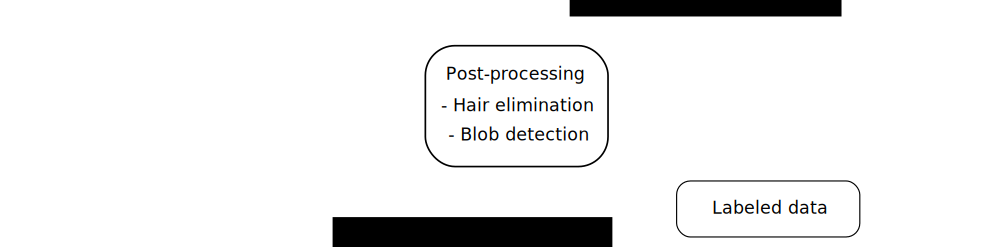
\includegraphics[width=\textwidth,height=\textheight,keepaspectratio]{flow_report}
 	\caption{Overview of the algorithm \label{fig:detection_flow}}
 \end{figure}
\FloatBarrier

\section{Data and annotation}

To evaluate the algorithm, a set of 106 images of faces en face were acquired from SCface database \cite{SCface} and FRGC database \cite{FRGC}. These images where collected at University of Zagreb and University of Notre Dame respectively. The purpose of the databases is to provide data to develop and improve face recognition algorithms. The images where taken in under controlled conditions indoor in a studio setting indoor with a high-quality photo camera. Figure \ref{fig:orig_img} shows a example of the images from the databases.

\FloatBarrier
\begin{figure}[h]
	\centering
	\includegraphics[width=\textwidth/2,height=\textheight/2,keepaspectratio]{001_orig}
	\caption{One example of the images used to evaluate the algorithm \label{fig:orig_img}}
\end{figure}
\FloatBarrier

Each image was examined the supervisors at NFC who labeled facial skin mark of interest. Each mark was given either the label permanent or non-permanent according to NFC definitions. This resulted in 506 marks where 353 were labeled as permanent and 153 non-permanent.

\section{Programing language}

The algorithm was implemented in Visual Studios 2013 using the OpenCV 3.0.0 \cite{opencv} for most image processing. The landmark detection algorithm comes from a open source library Dlib 18.18 \cite{dlib09}. When it comes to the graphs and bar-diagrams in this master thesis, Matlab \cite{MATLAB:2010} was used since it it easy to produce good looking graphs.   

\section{Pre-processing}

When the algorithm is given a RGB image, denoted $I$, it first detects the location of the face with the help of the face detector in OpenCV. It surrounds the face with a bounding box. With the bounding box, the facial landmark can be detected by using the algorithm from Dlib. This landmark algorithm was chosen since it reduces the error faster than other state of the art methods \cite{dlib_landmark}. 

\FloatBarrier
\begin{figure}[!h]
	\centering
	\includegraphics[width=\textwidth/2,height=\textheight/2,keepaspectratio]{landmarks}
	\caption{Image with the 64 landmarks shows as blue dots \label{fig:landmarks}}
\end{figure}
\FloatBarrier

With the landmarks, it is possible to begin the normalization process. First, the image is photometric normalized using LRSR algorithm. This tone mapping operator is fast and had a good implementation available in C++. It performs on pair with the best tone mapping operator of today \cite{badger}. Photometric normalization is vital since the visibility of facial marks can be affected by varying illumination of the image.  

Second, the image is rescaled such that the interpupillary distance is 500 pixels. This resizes the images to approximately 2100x2800 and the interpolation method used is cubic interpolation. The landmarks are also used to rotate the image so that the eyes are level. The rotation and resizing of the image is called geometric normalization and is necessary remove the effect of the distance and tilt of the camera. In \cref{fig:rotated_img} one can se the result from the image normalization. 

\FloatBarrier
\begin{figure}[!h]
	\centering
	\includegraphics[width=\textwidth/2,height=\textheight/2,keepaspectratio]{001_rotated}
	\caption{Image after photometric and geometric normalization \label{fig:rotated_img}}
\end{figure}
\FloatBarrier

The last part of the pre-processing step is to segment out areas which can cause false detections such as facial hair, nostrils, pupils etc. This is done by generating a binary mask. To segment out areas with skin, the implementation of GrabCut in OpenCV was used since it has proven to perform as well or better than many other user interactive foreground extraction methods \cite{grabcut}. From the skin mask, the eyes, nostrils, mouth and throat are cut out using elliptical shapes around the landmarks marking these regions. To expand these holes, a morphological erosion algorithm was performed on the image with a 3x3-kernel containing ones. The resulting mask can be observed in \cref{fig:mask_img}. 

\FloatBarrier
\begin{figure}[!h]
	\centering
	\includegraphics[width=\textwidth/2,height=\textheight/2,keepaspectratio]{001_mask}
	\caption{Image of the facial mask \label{fig:mask_img}}
\end{figure}
\FloatBarrier        

\section{Candidate detection}

The pre-processed image, denoted $I_{pre}$, can now be used to search for facial mark candidates. This is done with the help of FRS algorithm since it highlight circular shapes which can be more easily detected. The algorithm makes calculations with different radii, $N$, and the ones used are $N = \{1, 3, 5, 7, 9, 11, 13, 15 \}$. These radii was used since 75\% of facial marks had a area smaller than 600 pixels, see \cref{fig:result_box_size}. The Gaussian kernel $A_n$ size increased from 3x3 to 7x7 depending on the radius $r$. 

Below, \cref{fig:frs}, the resulting FRS image is presented. It is hard to see the facial marks since the image contains positive and negative values. By taking the absolute value of the the image, the marks appear more prominent, see \cref{fig:frs_abs}.  

\FloatBarrier
\begin{figure}[h]
	\centering
	\includegraphics[width=\textwidth/2,height=\textheight/2,keepaspectratio]{frs}
	\caption{FRS image \label{fig:frs}}
\end{figure}
\FloatBarrier

\FloatBarrier
\begin{figure}[h]
	\centering
	\includegraphics[width=\textwidth/2,height=\textheight/2,keepaspectratio]{frs_abs}
	\caption{Absolute value of FRS image \label{fig:frs_abs}}
\end{figure}
\FloatBarrier

At this point, an FRS-image with points of interest has been acquired. From this image, a binary threshold was applied with the threshold $h_{FRS}$, see \cref{eq:bin_thresh}.

\begin{equation} \label{eq:bin_thresh}
I(p) = 
\begin{cases}
1    & \quad \text{if } I(p) \geq h_{FRS} \: \text{max}(I) \\
0		& \quad  \text{ else}\\
\end{cases}
\end{equation}

This results in a binary image which is used in the watershed algorithm described by Fernand Meyer \cite{watershed}. The use of watershed is good since it can find the contour of uneven marks as long as the pixels approximately have the same intensity value. The watershed algorithm is applied on a gray image of the face. The output from this is a set of bonding boxes containing facial marks candidates.

The $h_{FRS}$ is the only parameter which is varied in the candidate detector. It is varied to examine the performance of the detector by looking at the recall and precision value of the detector. 

\section{Post-processing}

After candidate detection, the false detection was eliminated by using three methods. The first method finds candidates which contains a blob. The blob detector in OpenCV was used and it was given the three parameters: inertiaRatio, convexity and circularity. The method also allows to sort out all candidates which contains more than one blob. These candidates was eliminated.

%minInertiaRatio = 0 vs 1
%minconvexity = 0 vs 1
%minCircularit = 0 vs 1

The second part removes candidates which contain to many hair pixels. The $h_{hair}$ threshold was set to 0.02 and candidates containing more than 10\% hair pixels was excluded. 

The third and last method simply removed all candidates which had a larger area than 1000 pixels. This value was chosen since no annotated marks had a area larger than that, see \cref{fig:result_box_size}. 

\section{Classification}

When a set of facial marks has been acquired through the skin mark detector, they have to be separated into permanent and non-permanent marks. This is done with a non-linear SVM with a RBF-kernel. It was trained with different sets of feature descriptors, \cref{table:feature_sets}. Each set was trained with one part training data and evaluated with one part of test data.

The parameters $C$ and $\gamma$ was optimized by first training the classifier with a crude range of values. The $C$-value and $\gamma$ that gave the best accuracy from the crude grid of values was located. Next a finer grid search was performed in the region of the best pair of $C$ and $\gamma$. From this finer grid, the best parameters for the specific set of features could be picked out. Each grid of parameters contained 20x20 pair of parameters. The low amount of pair was chosen to reduce the computation time when searching for the best parameter pair.  

When in comes to the feature descriptors, the LBP-features has no variable parameters which is used in this master thesis. The HOG-features needs a couple of parameters. The window size was set to 48x48 pixels, block size was 8x8, block stride was 4x4, cell size 4x4 and 9 bins. 

The different set of features used to train the classifier can be seen in \cref{table:feature_sets}. Here, COLOR means the 11 color names described in \cref{subsection:Color}. 

\FloatBarrier
\begin{table}[h!]
	\begin{center}
		\caption{Sets of feature descriptors to be evaluated}
		\begin{tabular}{|c|l|}
			\hline
			Set &  Features   \\ \hline
			 1  &     RGB     \\ \hline
			 2  &     HSV     \\ \hline
			 3  &    COLOR    \\ \hline
			 4  &     HOG     \\ \hline
			 5  &     LBP     \\ \hline
			 6  &  HOG + RGB  \\ \hline
			 7  &  HOG + HSV  \\ \hline
			 8  & HOG + COLOR \\ \hline
			 9  &  LBP + RGB  \\ \hline
			 10  &  LBP + HSV  \\ \hline
			 11  & LBP + COLOR \\ \hline
			 12  & RGB + HSV + COLOR \\ \hline
		\end{tabular}
		\label{table:feature_sets}
	\end{center}
\end{table}
\FloatBarrier

\section{Evaluation}

To be able to compare the results from the different feature descriptors with each others it is crucial to have some kind of evaluation measurement. The most common measurements for binary classifiers are based on the confusion matrix \cite{sokolova2009systematic}. 

\subsection{Confusion matrix}

The confusion matrix displays the result from a classifier consist of four values:

\begin{itemize}
	\item True positive (TB)\\
	The samples which were labeled as class one has also been predicted to belong to class one.
	
	\item True negative (TN)\\
	The samples which were labeled as class two has also been predicted to belong to class two.
	
	\item False positive (FP)\\
	Samples that were incorrectly assigned to class one.
	
	\item False negative (FN)\\
	Samples that were incorrectly assigned to class two.
\end{itemize}

\FloatBarrier
\begin{figure}[!h]
	\centering
	\includegraphics[width=\textwidth*3/4,height=\textheight*3/4,keepaspectratio]{confusion_matrix.PNG}
	\caption{Confusion matrix
		\label{fig:confusion}}
\end{figure} 
\FloatBarrier

From the confusion matrix, a collections of performance measurement can be calculated. This master thesis will use three values: accuracy \cref{eq:accuracy}, precision \cref{eq:precision} and recall \cref{eq:recall}. Accuracy show the overall effectiveness of the classifier. Precision show class agreement of the data labels with the positive labels given by the classifier. Recall show the effectiveness of a classifier to identify positive labels

\begin{equation} \label{eq:accuracy}
\text{Accuracy} \: [\%] = \frac{\text{TP} + \text{TN}}{\text{TP}+\text{TN}+\text{FP}+\text{FN}}
\end{equation}

\begin{equation} \label{eq:precision}
\text{Precision} \: [\%] = \frac{\text{TP}}{\text{TP}+\text{FP}}
\end{equation}
\begin{equation} \label{eq:recall}
\text{Recall} \: [\%] = \frac{\text{TP}}{\text{TP}+\text{FN}}
\end{equation}

\subsection{Cross validation}

In order to avoid overfitting and get a reliable performance value, one often use a method called cross validation. Cross validation is when the data i split up into $k$-subsets an one of them is used as test data while $k -1$ are used as training data. See \cref{fig:cross_validation} for a schematic overview of a five-fold cross validations procedure.  


\FloatBarrier
\begin{figure}[!h]
	\centering
	\includegraphics[width=\textwidth*3/4,height=\textheight*3/4,keepaspectratio]{cross_validation.PNG}
	\caption{Cross validation
		\label{fig:cross_validation}}
\end{figure} 
\FloatBarrier

%To evaluate the detector and classifier, the performance values recall, precision and accuracy was used. For the detector, recall and precision was used to compare the performance of the $h_{FRS}$-value and the different elimination methods. For the classifier the accuracy measurement was used. A five-fold cross validation was used throughout the evaluation of the classifier.   






























%\subsection{Facial grid}
%
%The landmarks are also used to produce a grid over the face. The grid consist of 16 regions which are defined the supervisors at NFC. This grid is needed to calculate the number of facial marks within these predefined regions. This is necessary to improve the evidential value of the likelihood ratio.
%
%\begin{figure}[h!]
%	\centering
%	\includegraphics[width=\textwidth/2,height=\textheight/2,keepaspectratio]{001_grid}
%	\caption{Image over the landmarks (blue points) and facial grid (black lines) \label{fig:grid_img}}
%\end{figure}
%
%\section{Classification}
%
% Generally, support vector machine (SVM) tend to perform better with continuous and multidimensional features and with a large amount of samples. The features used in this case fulfill the continuity and multi dimension. Chih-Wei et. al. \cite{svm_guide} also describes a good way to optimize the use of SVM and recommend to use radial basis function (RBF) as kernel. This is why a SVM with RBF kernel is chosen for the mark classifier.  
%
%The goal with a SVM is to separate different classes by finding the best hyperplane which divides them. The hyperplane is moved such that a loss-function is minimized. RBF kernel nonlinearly maps samples into a higher dimensional space which allows the classifier to handle non-linearly separable classes. This kernel also has fewer numerical difficulties. The parameters needed for a RBF kernel i $C$ which determines the penalty parameter for the error and $\gamma$ which defines how far the influence of a single training sample reaches. \cite{svm_guide}
%
%The training data consists of the labelled facial marks provided by the supervisors at NFC. To get a good classifier, a set of discriminative features are required.
%
%\subsection{Features}
%
%The most common color space in use is the RGB system, one channel each for the red, green and blue colors. Arfika Nurhudatiana et al. \cite{torso_RPPVSM} used, among others, the minimum, maximum, and average from the RGB-channels as discriminative features. 
%
%The features extracted from the facial marks are the mean and the standard deviation from the three RGB channels and the 11 colours from the work of Joost van de Weijer et al. This results in 28 features which is used to train the classifier. 
%
%To not let some feature with greater numeric rang dominate over features with smaller range, the features need to be scaled \cite{svm_guide}. This is very important which is why the features are linearly scaled to a range from $0$ to $1$. The same scaling factor has to be used when the test data is scaled. 






  

\chapter{Result}\label{cha:result}

This Chapter first describes the experiment to evaluate the algorithm and then presents the results.

\section{Experiment}
%{and FRGC database CITE}
To evaluate the algorithm, a set of 106 images of faces en face were acquired from SCface database \cite{SCface}. Facial marks of interest were marked and labeled as a permanent or a non-permanent by the supervisors at NFC. This resulted in 506 marks where 353 were permanent and 153 were non-permanent.

The experiment was set such that the image set was processed by the algorithm with 11 different thresholds values, $h_{FRS}$, for the FRS-image. The $h_{FRS}$ ranged from $0.05$ to $0.15$. The output was compared to the ground truth. A correct detection was defined as all detections which had a union with an annotated mark. This definition has been chosen since some of the detections can be very small. Also, since candidates larger than 1000 pixels has been eliminated, no over large candidates can give correct detections.   

The evaluation measurement for the detector is the precision \eqref{eq:precision} and recall \eqref{eq:recall} value. Precision tells how well the detector is to avoid false detections while recall tells how well it finds the annotated marks. The result from the different $h_{FRS}$-values can be seen in \cref{fig:results_bar_frs}.

\begin{equation} \label{eq:precision}
Precision = \frac{\text{Number of correct detections}}{\text{Number of detections}}
\end{equation}
\begin{equation} \label{eq:recall}
Recall = \frac{\text{Number of correct detections}}{\text{Number of annotated marks}}
\end{equation}

The $h_{FRS}$-value which gives the best recall value was used to evaluate the elimination process of the candidates. This was done by calculating the precision and recall values before the different elimination steps. The results is displayed in \cref{fig:results_bar_frs}.

To evaluate the facial mark classifier, a cross validation of the 506 annotated mark were performed. 25 marks was chosen at random to be used as test marks while the remaining marks was used for training the SVM. This was repeated until all the marks had been used as test marks.

In order to find the best $C$-value and $\gamma$-value for the mark classifier, the parameters are varied over a rough interval to narrow down the search. Afterwards, a more fine interval is used to find the best parameters. This has been shown by Chih-Wei et. al. \cite{svm_guide}  to be an effective method compared to a more random selection of parameters which is often used by people unfamiliar to SVM. 

\section{Results from experiment}

In the \cref{fig:results_bar_frs}, the precision and recall for different $h_{FRS}$-value can be examined. The precision corresponds to the white bar and the recall corresponds to the black bar. Note that this is only the detections of facial mark and no classification between permanent and non-permanent marks. 

\begin{figure}[h!]
	\centering
	\includegraphics[width=\textwidth*3/4,height=\textheight*3/4,keepaspectratio]{results_bar_frs}
	\caption{Detection results from the algorithm with different $h_{frs}$-values. The white bars represent the precision value and the black bars represent recall value.  \label{fig:results_bar_frs}}
\end{figure}

As one can see, the precision increases with higher $h_{FRS}$-value without affecting the recall substantially. This is means that the number of candidates decreases with a growing $h_{FRS}$-value. Thus, a small $h_{FRS}$-value results in a large amount of candidates while a larger value gives fewer candidates.

In \cref{fig:results_bar_elimniation}, it is possible to see the effects of the different elimination steps. As before, the white bar represent the precision and the black bar represent the recall. The first pair is the result just after the candidate detection and the second pair is the result after the blob detector. Furthermore, the third pair is after the hair eliminator and the last pair is after the size eliminator. 

\begin{figure}[h!]
	\centering
	\includegraphics[width=\textwidth*3/4,height=\textheight*3/4,keepaspectratio]{results_bar_elimniation}
	\caption{Detection results from the algorithm  after different candidate elimination steps. 1 = before elimination, 2 = after blob-elimination, 3 = after hair-elimination, 4 = after size-elimination. The white bars represent the precision value and the black bars represent recall value.  \label{fig:results_bar_elimniation}}
\end{figure}

It is obvious that the different eliminators are essential for the algorithm. The hair eliminator improves the precision the most while the blob detector worsen the recall the most.     




%The result from the classifier can be presented as a confusion matrix, see \cref{table:confusion_mat}. A positive result is a permanent mark and a negative result is a non-permanent mark. The accuracy of the classifier is $83\%$ 

%\begin{table}[h!]
%\begin{center}
%	\caption{Confusion matrix from RPPVS classifier}
%	\begin{tabular}{|c|c|c|}
%		\hline
%		                 & Predicted positive & Predicted negative \\ \hline
%		Labeled positive &        321         &        32         \\ \hline
%		Labeled negative &         54         &        99         \\ \hline
%
%	\end{tabular}
%
%\label{table:confusion_mat}
%\end{center}
%\end{table}
\newpage
The result from the mark classifier is presented as accuracy matrix with varying $C$-value and $\gamma$-value. The accuracy is calculated as in \eqref{eq:accuracy}. In \cref{fig:crude_acc}, the $C$-value ranges from $1$ to $100$ while the $\gamma$-value ranges from $10^{-2}$ to $1$.

\begin{equation} \label{eq:accuracy}
Accuracy [\%] = \frac{\text{True positive} + \text{True negative}}{\text{Number of annotated marks}}
\end{equation}

\begin{figure}[h!]
	\centering
	\includegraphics[width=\textwidth*3/4,height=\textheight*3/4,keepaspectratio]{crude_acc_2}
	\caption{Crude accuracy matrix where $1 \leq \gamma \leq 100$ and $10^{-2} \leq \gamma \leq 1$.
		 \label{fig:crude_acc}}
\end{figure}

 As show, the best accuracy is when $C \approx 95$ and $\gamma \approx 5*10^{-2}$. Therefore, with a finer interval for the two parameters, \cref{fig:fine_acc} was generated. Here, the $C$-value ranges from $90$ to $115$ while the $\gamma$-value ranges from $5*10^{-2}$ to $2*10^{-1}$. 

\begin{figure}[h!]
	\centering
	\includegraphics[width=\textwidth*3/4,height=\textheight*3/4,keepaspectratio]{fine_acc_2}
	\caption{Fine accuracy matrix where $90 \leq \gamma \leq 115$ and $5*10^{-2} \leq \gamma \leq 2*10^{-1}$.
		 \label{fig:fine_acc}}
\end{figure}

Form \cref{fig:fine_acc} it is possible to conclude that the best accuracy is acquired with several pair of parameters and results in the accuracy 90\%. $C = 100$ and $\gamma = 0,14$ is one of those pairs. Therefore, the mark classifier is given these values as parameters for the SVM. 




\chapter{Discussion}\label{cha:Discussion}

This section will discuss the results from the algorithm and the methods used to implement it.

\section{Result}

As seen, the detector has problem with false detections which is a huge problem. The precision is not very good, not even over 10\%, due to the many false detections. The precision does not increase faster than the decline of the recall with an increasing $h_{frs}$-value. This indicates that there are margins for improvement when it comes to the candidate detector. The elimination method used does improve the precession well enough which means that they also can be improved.

When looking at the accuracy of the mark classifier, with an accuracy of 90\%, the result is pretty satisfactory. 


\section{Method}

There are a lot to say about the methods used in the algorithm. The major problem with the algorithm is the elimination of candidates. The blob detector works well in not eliminating true detections which the hair removal algorithm does not. It eliminates candidates which are true facial marks. This is because it indicates that the facial marks are hair which makes it hard to separate the true candidates and the hair intensive candidates. 
Tim et Lee al. describes their algorithm well except when they are explaining how to calculate the hair mask for each colour channel. It is not clear what the maximum from refers to. The algorithm in this work used the maximal pixel value between the different structuring elements. 

The mark detector used in the algorithm was good at indicating the potential facial marks but the simple thresholding method to pin point them out was not optimal. It kept the pixels larger than a certain percent of the maximal value in the FRS image. This resulted in many unnecessary candidates which of course contributed to the high false detection rate. 

The blob-detector used is hardly improving the precision at the cost of recall loss. This means that the blob-detector is not contributing to the algorithm in a positive way. The hair-eliminator on the other hand does improve the precision which is the whole point with the candidate eliminators.  

When it comes to the mark classifier, it could have performed better if the number of features was larger and more explored. Now the features are very simple and there is overweight of permanent marks among the annotated facial marks which is not ideal.

Regarding the references used in these thesis, several of them uses FRS to detect point of interest which shows the actuality of the method. Many of the papers trying to detect facial marks uses a crude segmentation mask which does not follow the hairline and chin well. This algorithm uses a more precise segmentation method which reduces the areas which is not processed. 


\section{Ethical perspective}

As with all applications which can be used for surveillance of people, the integrity is at stake. Facial recognition algorithms using facial marks can be misused for malicious intent. They can also help the legal system to catch and convict criminals which is desirable outcome of this paper. 

When it comes to the facial images, they are taken from a open source database which should only be used for academical research. There are no personal information attached to the images which makes them as anonymous as possible without corrupting the images.    

\chapter{Conclusion}\label{cha:conclusion}

This master thesis has examined the possibilities to develop an algorithm which could detect facial marks and separate them into permanent and non-permanent. The result from the experiments shows that the detector can initially find the facial mark with high recall but with a low precision. The precision increases as the false detections are eliminated. The mark classifier demonstrates good result with its accuracy of 90\%.  

A proposed remedy for the low precision on the detector is to improve the elimination of the false candidates. The hair-detector is to crude and may be combined with or replaced by a module which looks at the Fourier Transform of the candidates. The mark classifier could perform better with better discriminative features. By finding better features through examination of the differences between permanent and non-permanent marks.


%% End of the body 


	
\newpage
\bibliographystyle{unsrt} %Style which sort after referenced 
\bibliography{references}
	
	%% End of the document
	
\end{document}